\documentclass{article}
\usepackage{amsmath}
\usepackage{graphicx}
\usepackage[utf8]{inputenc}
\usepackage[T1, T2A]{fontenc}
\usepackage[english,russian]{babel}

\title{Задачи к теорминимуму}
\author{Anikin Evgeny, 121}

\begin{document}
	\maketitle
	\section{Средняя скорость}
	Средняя скорость в зависимости от $v_0$:
	\begin{equation}
		\overline{v}  =	\frac{\pi R \sqrt{a}}{2K(\sqrt{b/a})} 
		= \frac{\pi\sqrt{v_0^2 + {\displaystyle \frac{\epsilon(gR + v_0^2)}{\lambda + 1}}}}
				{2 K\!\left(\sqrt{
				{\displaystyle \frac{2\epsilon(gR + v_0^2)}{(\lambda + 1) v_0^2 + 
												\epsilon(gR + v_0^2)}}
				}\right)}
	\end{equation}
	Для коэффициента трения имеем
	\begin{equation}
		k > \frac{\epsilon}{3} 
			\frac{|2gR - v_0^2|}{\sqrt{(gR)^2 - (2\epsilon v_0^2)^2}} + O(\epsilon^2),
	\end{equation}
	График в координатах $\overline{v}$, $k$:
	\begin{figure}[ht]
		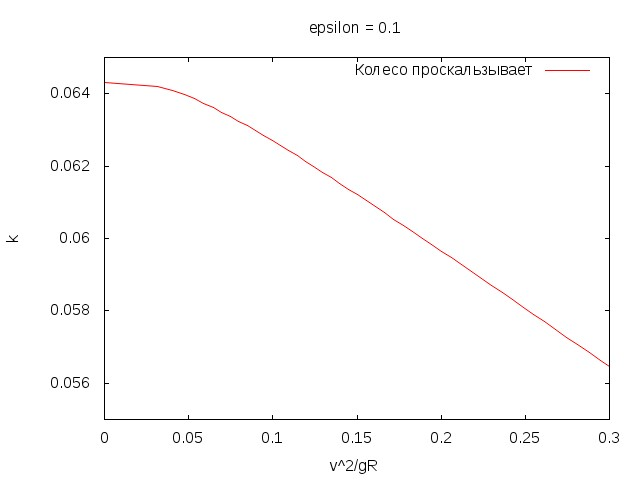
\includegraphics[width=\linewidth]{overv.jpg}
	\end{figure}
	
	\section{Как найти среднюю скорость}
	Угловая скорость колеса зависит от угла так:
	\begin{equation}
		\omega^2 = \frac{2(E/m - gy)}{I/m + y^2 + \xi^2}
	\end{equation}
	В первом порядке по $\epsilon$ получается так:
	\begin{equation}
		\omega^2 = \frac{v_0^2}{R^2} - \frac{gR + v_0^2}{(\lambda + 1)R^2}
			\epsilon\cos{2\alpha}
	\end{equation}
	Здесь
	\begin{equation}
		v_0^2 = \frac{2(E - mgR)}{m + I/R^2},	
	\end{equation}	
	\begin{equation}
		I = \lambda mR^2
	\end{equation}
	Можно сделать замену $\alpha = \beta + \pi/2$, тогда выражение выше приводится к 
	\begin{equation}
		\label{diffeq}
		\omega^2 = a - b\sin^2{\beta}
	\end{equation}
	где
	\begin{equation}
		a = \frac{v_0^2}{R^2} + \epsilon \frac{gR + v_0^2}{R^2(\lambda + 1)}
	\end{equation}
	\begin{equation}
		b = 2\epsilon\frac{gR + v_0^2}{R^2(\lambda + 1)}
	\end{equation}

	Решив уравнение \ref{diffeq}, можно найти время, которое проходит между положениями неустойчивого
	равновесия.
	Средняя скорость получается такой:
	\begin{equation}
		\label{vv0}
		\overline{v}  =	\frac{\pi R \sqrt{a}}{2K(\sqrt{b/a})} 
		= \frac{\pi\sqrt{v_0^2 + {\displaystyle \frac{\epsilon(gR + v_0^2)}{\lambda + 1}}}}
				{2 K\!\left(\sqrt{
				{\displaystyle \frac{2\epsilon(gR + v_0^2)}{(\lambda + 1) v_0^2 + 
												\epsilon(gR + v_0^2)}}
				}\right)}
	\end{equation}
	Здесь $K(x)$ --- полный эллиптический интеграл первого рода.
	Легко видеть, что если $v_0 \gg \epsilon gR$, то $\overline{v} \approx v_0$.

	Для максимального коэффициента трения была ранее получена формула
	\begin{equation}
		\label{kv0}
		k > \frac{\epsilon}{3} 
			\frac{|2gR - v_0^2|}{\sqrt{(gR)^2 - (2\epsilon v_0^2)^2}} + O(\epsilon^2),
	\end{equation}

	Теперь можно построить график зависимости $k$ от $\overline{v}$, он задаётся параметрически
	формулами \ref{kv0} и \ref{vv0}.
\end{document}
